\documentclass{beamer}
\usepackage[latin1]{inputenc}

\usepackage[noend]{algpseudocode}
\usepackage[ruled]{algorithm}
\usepackage{url}
\usepackage{framed}
\usepackage{amsfonts,amsmath,amsthm}
\usepackage{graphicx}
\usepackage{url}
\usepackage{color}

\title{Rational Monte Carlo Tree Search}
\author{David Tolpin, Solomon Eyal Shimony}
\institute{Ben-Gurion University of the Negev\\Beer Sheva, Israel}
\date{June 1, 2011}

\AtBeginSection[]
{
  \begin{frame}<beamer>
    \frametitle{Outline}
    \tableofcontents[currentsection]
  \end{frame}
}


\begin{document}

\begin{frame}
\titlepage
\end{frame}

\begin{frame}{UCT}
UCT (Upper Confidence Bounds on Trees) is popular for Monte
  Carlo search in large trees:
\begin{itemize}
\item Selects an action $a_i$ that maximizes $\overline r_i + C\sqrt
  {\frac {\log n} {n_i}}$
\item Chooses a non-optimal action $n_i\ge\rho\log n$ times ($\rho$ is
  some constant).
\item Based on UCB1, that achieves logarithmic regret for multi-armed
  bandits.
\item But {\bf{\Large no bandits in Monte Carlo:}} {\bf no reward} is given for {\bf
  sampling} a good action.
\end{itemize}
\end{frame}

\begin{frame}{Doing better than UCT on sets}
\begin{figure}[h]
\centering
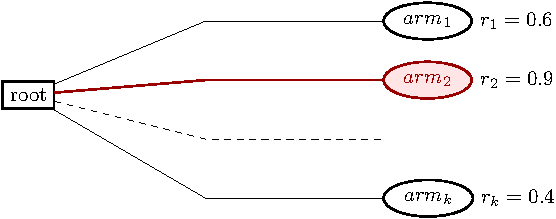
\includegraphics[scale=0.8]{onelevel-tree.pdf}
\end{figure}
When an arm is selected based on the {\bf sample mean}:
\begin{itemize}
\item Regret of UCB decreases {\it polynomially} with $n$.
\item Regret of $\epsilon$-greedy decreases {\it exponentially} with
  $n$.
\item Regret of UVB: $\max V_i$, $V_{i_{best}}=\frac {1-1/k}
  {n_{i_{best}}},\quad V_{i_{other}}=\frac {1/k} {n_{i_{other}}}$
  decreases exponentially with $n$, faster than $\epsilon$-greedy.
\end{itemize}
\end{frame}

\begin{frame}{UCB vs. $\epsilon$-greedy vs UVB}
\begin{figure}[h]
\centering
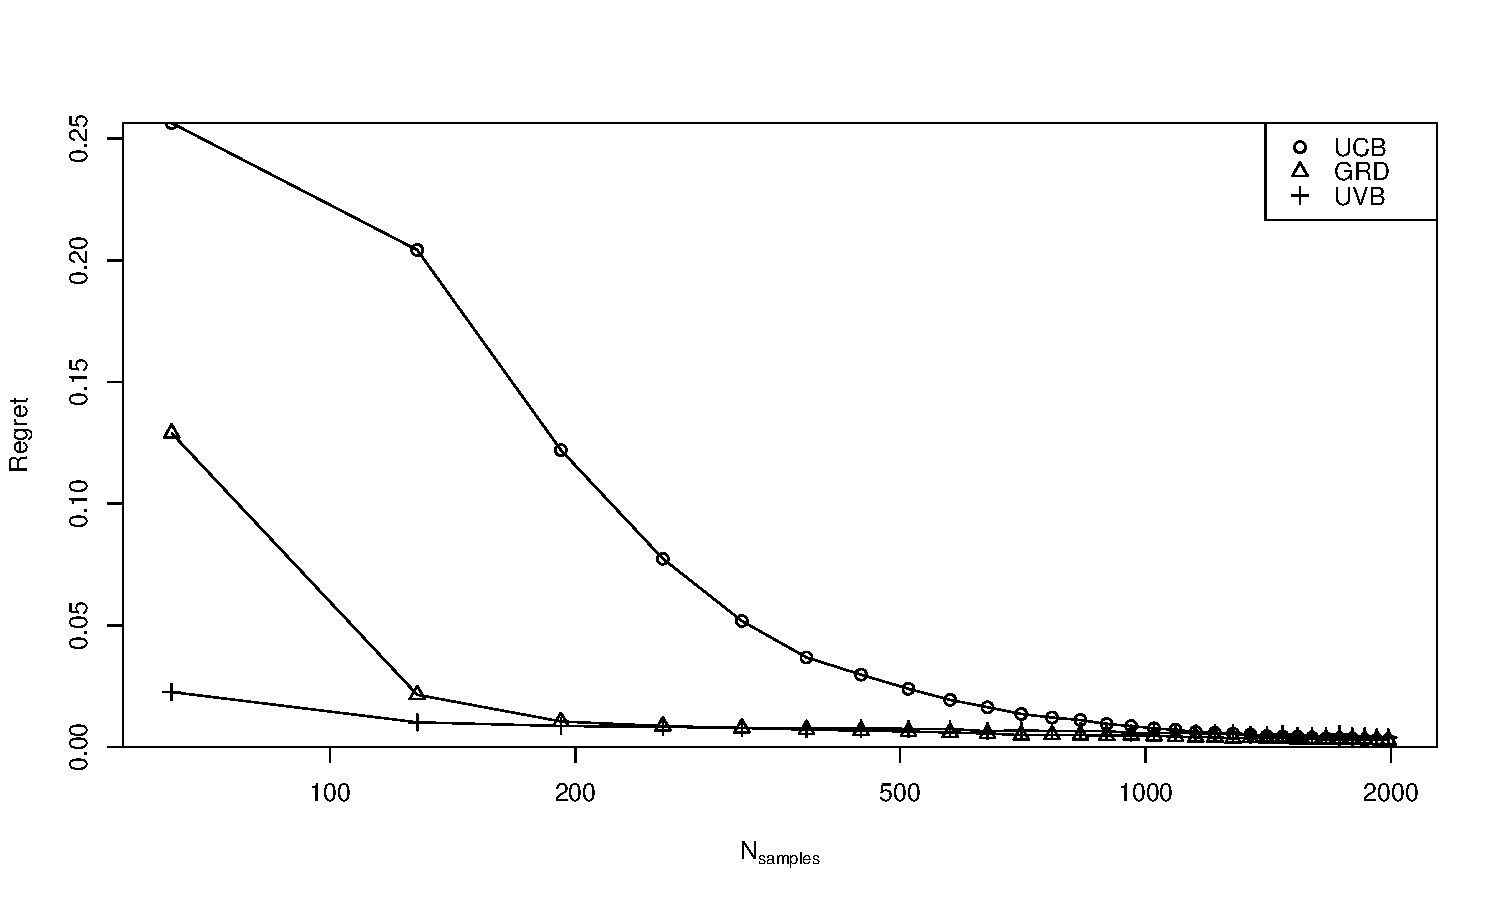
\includegraphics[scale=0.45]{onelevel-64.pdf}

64 Bernoulli arms, randomly generated
\end{figure}
\end{frame}

\begin{frame}{Doing Better Than UCT on Trees}
Uniform sampling is useless in this tree:
\begin{figure}[h]
\centering
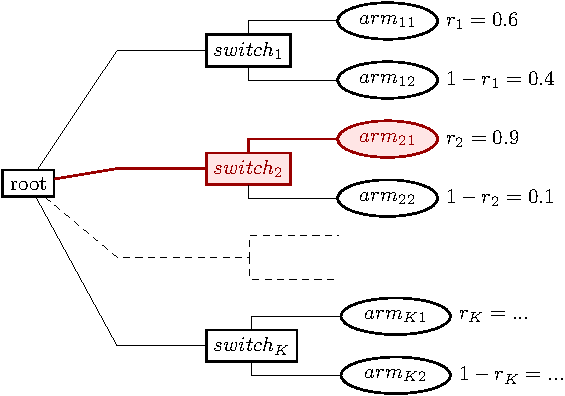
\includegraphics[scale=0.8]{twolevel-tree.pdf}
\end{figure}
Rational sampling:
\begin{itemize}
\item first, choose an action that maximizes VOI (UVB);
\item then, choose actions that maximize average reward (UCB).
\end{itemize}
\end{frame}{}

\begin{frame}{UVT vs. VCT (UVB+UCT) vs. UCT}
\begin{figure}[h]
\centering
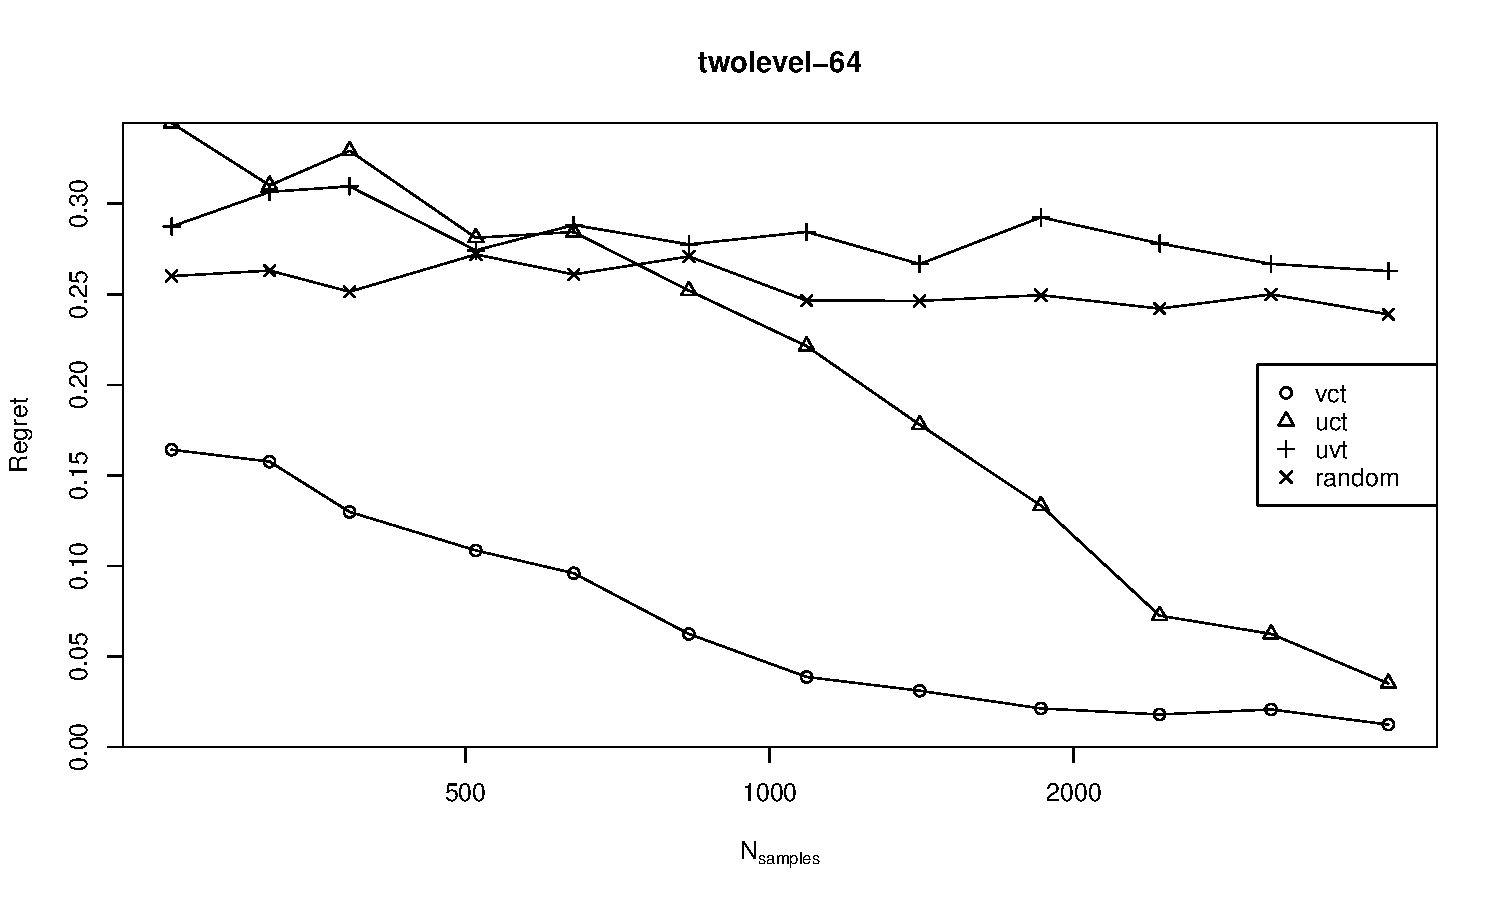
\includegraphics[scale=0.45]{twolevel-64.pdf}

64 Bernoulli arms, randomly generated
\end{figure}
\end{frame}

\end{document}
